\section{Разработка корпуса}
\label{sec:case}

\subsection{Выбор программного обеспечения}
\subsubsection{AutoCAD}
AutoCAD — двух- и трёхмерная система автоматизированного проектирования и черчения, разработанная компанией Autodesk. Первая версия системы была выпущена в 1982 году. AutoCAD и специализированные приложения на его основе нашли широкое применение в машиностроении, строительстве, архитектуре и других отраслях промышленности.


Ранние версии AutoCAD оперировали небольшим числом элементарных объектов, такими как круги, линии, дуги и текст, из которых составлялись более сложные. В этом качестве AutoCAD заслужил репутацию «электронного кульмана», которая остаётся за ним и поныне. Однако на современном этапе возможности AutoCAD весьма широки и намного превосходят возможности «электронного кульмана».


В области двумерного проектирования AutoCAD по-прежнему позволяет использовать элементарные графические примитивы для получения более сложных объектов. Кроме того, программа предоставляет весьма обширные возможности работы со слоями и аннотативными объектами (размерами, текстом, обозначениями). Использование механизма внешних ссылок (XRef) позволяет разбивать чертёж на составные файлы, за которые ответственны различные разработчики, а динамические блоки расширяют возможности автоматизации 2D-проектирования обычным пользователем без использования программирования. Начиная с версии 2010, в AutoCAD реализована поддержка двумерного параметрического черчения. В версии 2014 появилась возможность динамической связи чертежа с реальными картографическими данными (GeoLocation API).

\subsubsection{Blender}

Blender — профессиональное свободное и открытое программное обеспечение для создания трёхмерной компьютерной графики, включающее в себя средства моделирования, скульптинга, анимации, симуляции, рендеринга, постобработки и монтажа видео со звуком, компоновки с помощью «узлов» (Node Compositing), а также создания 2D-анимаций. В настоящее время пользуется большой популярностью среди бесплатных 3D-редакторов в связи с его быстрым стабильным развитием и технической поддержкой.


Характерной особенностью пакета Blender выступает его небольшой размер по сравнению с другими популярными пакетами для 3D-моделирования. Документация в поставку не входит, но доступна онлайн. Демонстрационные сцены можно скачать на официальном сайте или на сайте открытых проектов «Blender Cloud». 


Blender имел репутацию программы, сложной для изучения. Практически каждая функция имеет соответствующее ей сочетание клавиш. Учитывая количество возможностей, предоставляемых Blender, каждая клавиша включена в более чем одно сочетание (shortcut). С тех пор как Blender стал проектом с открытым исходным кодом, были добавлены полные контекстные меню ко всем функциям, а использование инструментов сделано более логичным и гибким. С последующим улучшением пользовательского интерфейса были введены цветовые схемы, прозрачные плавающие элементы, а также новая система просмотра дерева объектов и другие различные мелкие изменения.

\subsubsection{SolidWorks}

Программное решение SOLIDWORKS 3D CAD предназначено для инженеров-конструкторов, инженеров-технологов и промышленных дизайнеров. Оно помогает проектировать инновационные промышленные изделия, проводить их виртуальные испытания, выполнять подготовку к производству, управлять инженерными данными и взаимодействовать на протяжении всего рабочего процесса. Все продукты семейства SOLIDWORKS работают в той же среде, что и SOLIDWORKS 3D CAD, и полностью интегрированы с этим продуктом. Это означает, что все специалисты работают с одними и теми же данными; любое изменение автоматически отражается во всех приложениях.

\begin{itemize}
    \item Проектные и производственные подразделения работают параллельно в одной и той же интегрированной системе.
    \item Изменения можно вносить на любой стадии, и они сразу же становятся доступны всем участникам процесса.
    \item 3D-модели и 2D-чертежи деталей и изделий любой сложности создаются быстро и с высокой точностью.
    \item Эффективность обеспечивается благодаря специализированным функциям для работы с отверстиями, крепежными элементами, деталями из листового материала, литьевыми формами, литыми (в том числе пластмассовыми) деталями, сварными швами, поверхностями, сетчатыми моделями, трубопроводами
    и электрическими кабелями, а также возможностям обратного проектирования.
    \item С файлами большинства 3D-систем можно работать в их исходном формате; существует также возможность автоматического преобразования таких файлов в формат SOLIDWORKS.
\end{itemize}

\subsubsection{Окончательный выбор}
Изучив представленные программы и другие альтернативы, был сделан выбор в пользу программы SolidWorks, ввиду ее возможности интеграций со сторонним программным обеспечением (в т.ч. Altium Designer), большому количеству бесплатных обучающих видеоматериалов\cite{sw_docs}, а так же возможности проведения симуляций.

\subsection{Моделирование корпуса}
Корпус системы является важным элементом, который обеспечивает ее защиту от внешних воздействий, а также удобство использования. Корпус должен быть изготовлен из прочных материалов, устойчивых к механическим повреждениям и воздействию окружающей среды.

К необходимым в корпусе элементам можно отнести
\begin{itemize}
    \item Посадочные отверстия для платы;
    \item Отверстие для силового разъема;
    \item Отверстие под рокер питания;
    \item Отверстие под вывод шлейфа;
    \item Отверстие под разъем I2C.
\end{itemize}

На скриншотах, приведенных ниже, показаны этапы разработки модели корпуса системы. Для того, что бы смоделировать корпус необходимо импортировать 3D модель печатной платы с элементами в \textit{САПР}. Для этого был выбран формат STEP, как формат, который поддерживается в обоих средах разработки. 

\begin{figure}[ht]
    \centering
    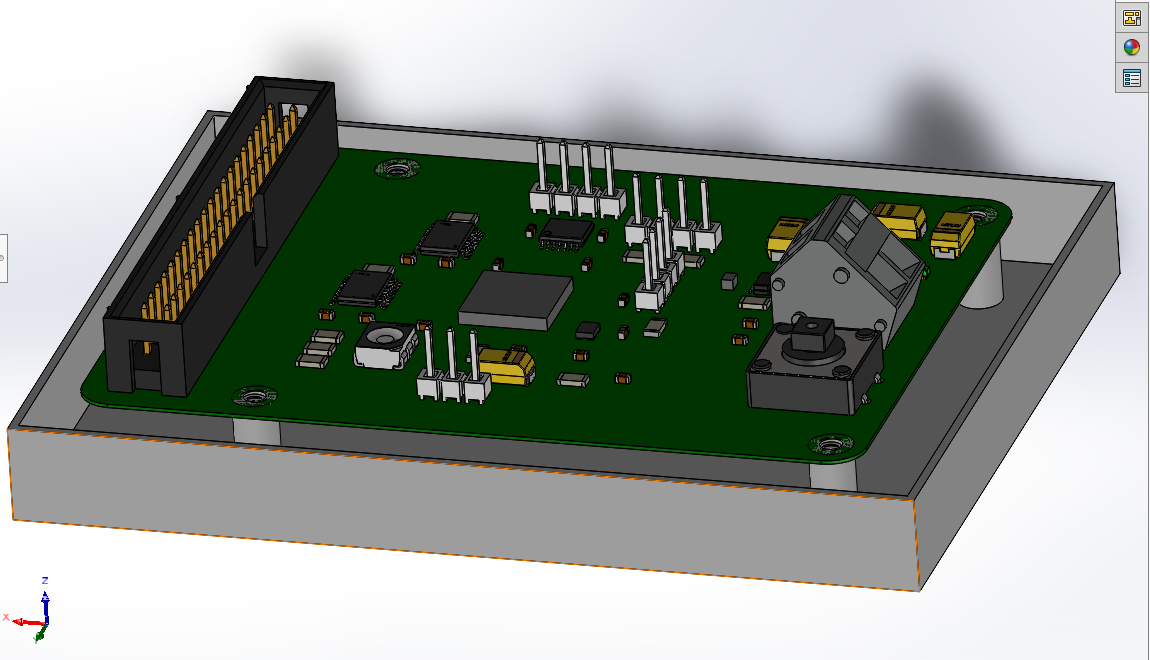
\includegraphics[width=0.6\linewidth]{\commonSecPathPrefix/sec_8/content/pcb_and_case.png}
    \caption{Посадочные стойки для платы}
\end{figure}

Далее последовал этап моделирования основы для платы -- пластиковые основы и резьбой под винт M3, используемый для крепления платы.
Фото печатной платы и посадочных ножек в разрезе показано ниже:
\begin{figure}[ht]
    \centering
    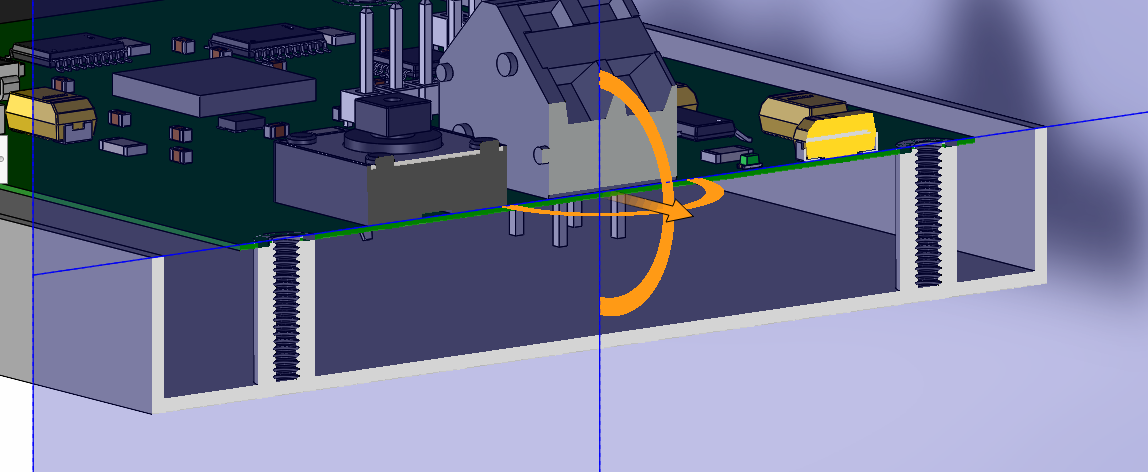
\includegraphics[width=0.7\linewidth]{\commonSecPathPrefix/sec_8/content/slice.png}
    \caption{Разрез основания под плату и стоек}
\end{figure}

После этого были добавлены отверстия под шлейф, I2C, разъем питания. Для этого использовались булевые операции над 3D объектами, редактирование чертежа и последующая его экструзия.

После заверешения этапа моделирования необходимо определить материал для корпуса. Так как условия допускают небольшие перепады температуры, а так же потенциальное наличие агрессивных сред (испарения флюса), то было приято решение использовать \textit{ABS} пластик. Для 3D печати необходимо подготовить GCODE файл, который содержит инструкции для 3D принтера. После экспорта модели из SolidWorks, был использован слайсер "\textit{Simplify3D}".
\begin{figure}[ht]
    \centering
    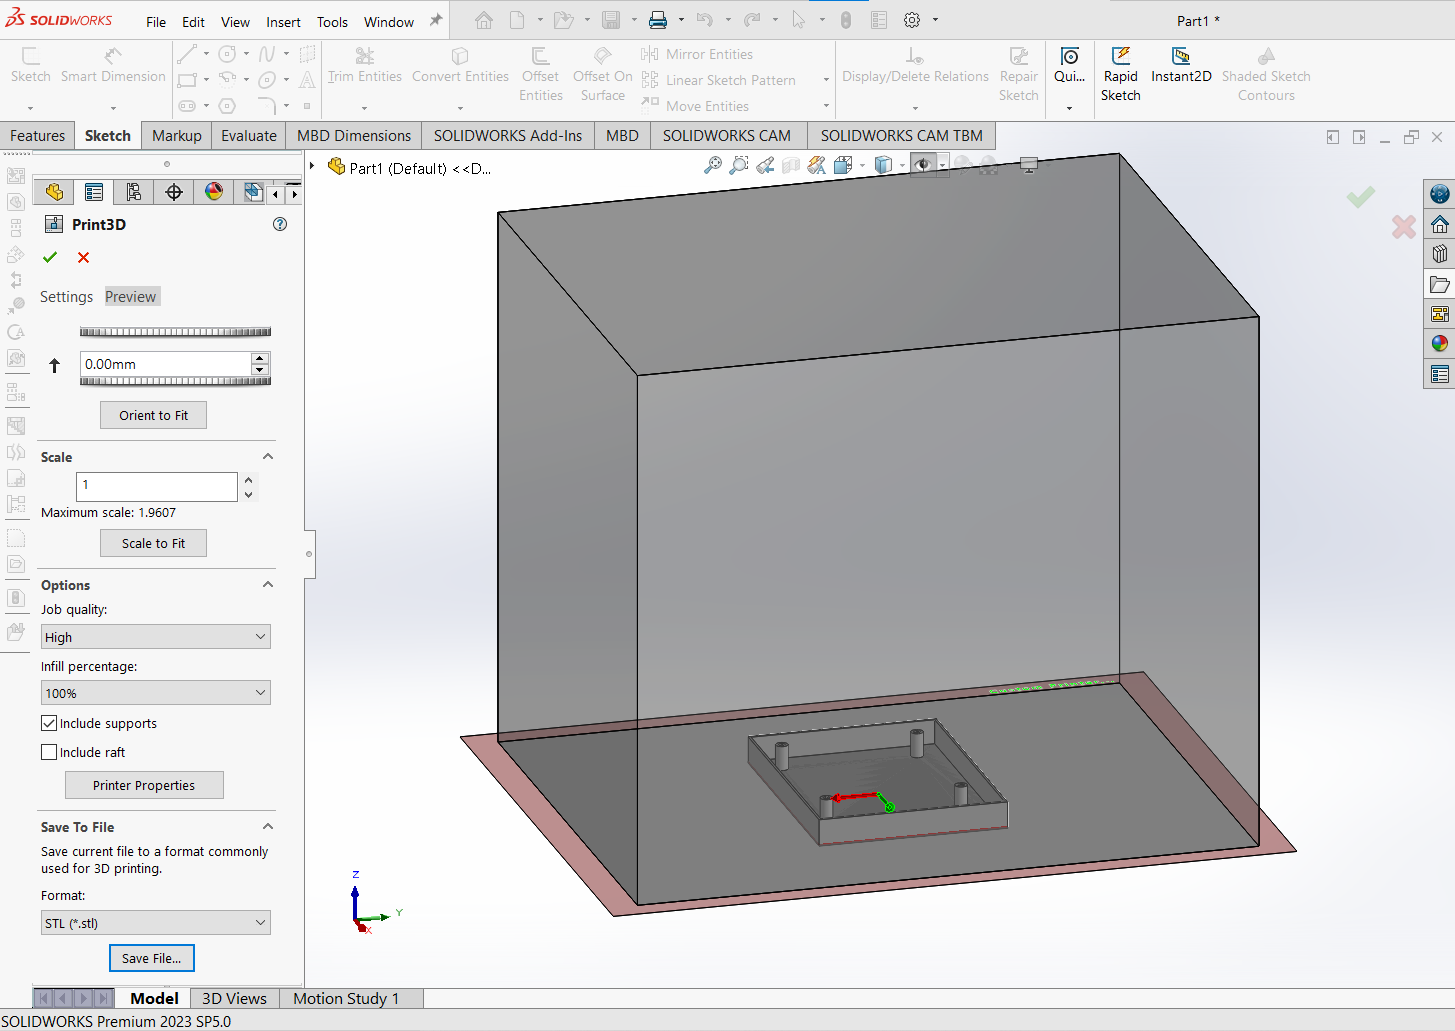
\includegraphics[width=0.6\linewidth]{\commonSecPathPrefix/sec_8/content/3d_printing.png}
    \caption{Разрез основания под плату и стоек}
\end{figure}

После печати корпуса необходимо произвести контрольные замеры габаритных и посадочных отверстий, осмотреть корпус на предмет дефектов печати. После этого происходит этап сборки устройства.